\chapter*{Introducción}
En el año 1758, Euler publica un artículo que cubre diversas propiedades de
los poliedros. El principal resultado de su artículo es la celebrada fórmula
de Euler para poliedros convexos,
\[V-A+C=2\]
La demostración de este resultado se basa en el hecho de que los poliedros
convexos son homeomorfos a un sólido común, la bola cerrada. Si consideramos
un poliedro irregular que sea homeomorfo a la esfera, este resultado sigue
siendo válido.

Sin embargo, podemos encontrar poliedros que no verifiquen esta fórmula
eliminando la condición de convexidad. Un ejemplo de poliedro que no verifica
esta expresión es el tetrahemihexaedro, con 6 vértices, 12 aristas y 7 caras.
Si computamos su valor $V-A+C$, obtenemos
\[6-12+7=1\]
El valor $V-A+C$ de un poliedro regular se denomina \emph{característica de
Euler} del poliedro.

\begin{marginfigure}
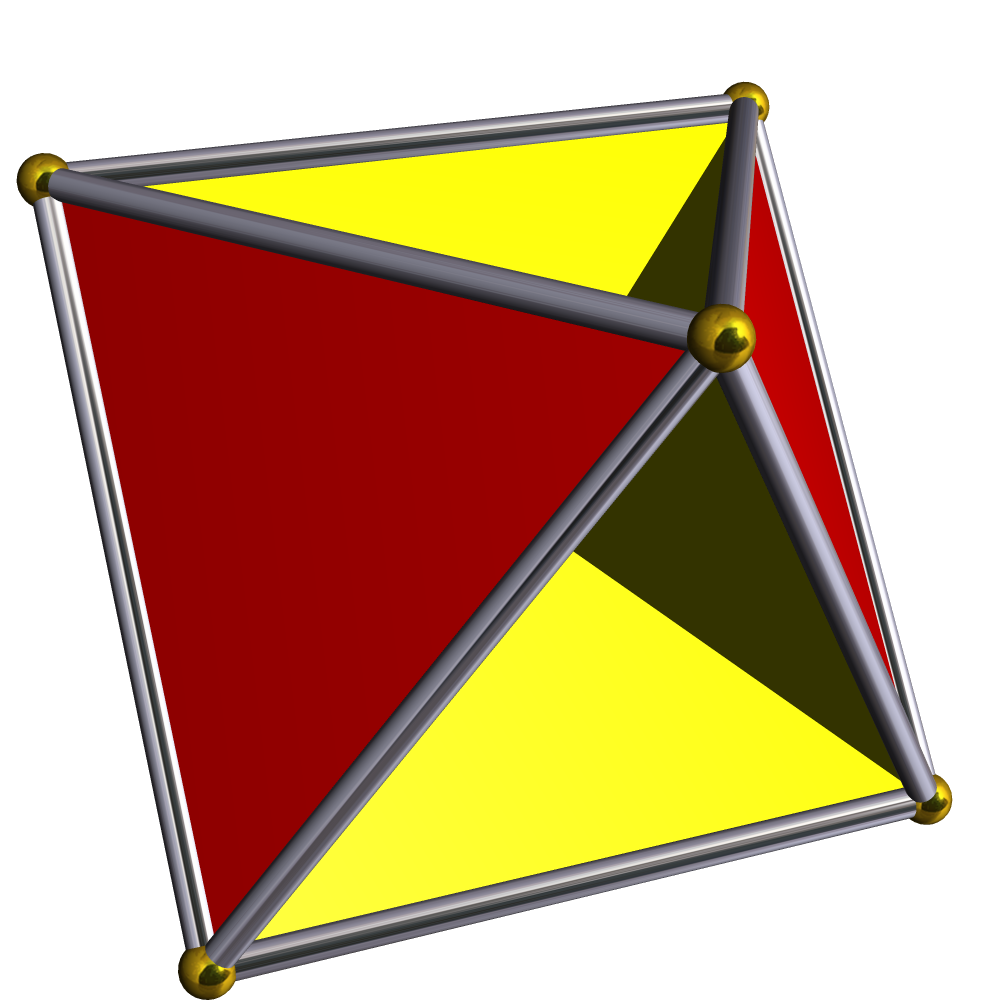
\includegraphics{Figures/Tetrahemihexahedron.png}
%https://en.wikipedia.org/wiki/Euler_characteristic#/media/File:Tetrahemihexahedron.png
\caption[Tetrahemihexaedro]{Tetrahemihexaedro regular. Algunas de sus caras se
intersecan entre sí, haciendo que su topología sea diferente a la de la bola
cerrada. Imagen: \cite{Tetra}.}
\end{marginfigure}

Un espacio topológico $X \subset \mb{R}^n$ 2AN y Hausdorff es una superficie
si, dado $p \in X$, existe un entorno abierto $U \subset X$ de $p$ homeomorfo
a una bola de $\mb{R}^2$. Desde un punto de vista geométrico, podemos decir
que los puntos de $X$ perciben el mundo en dos dimensiones, al igual que los
personajes de la novela \emph{Planilandia}. Algunas superficies pueden ser
representadas utilizando poliedros regulares, que podemos clasificar en
función de su característica de Euler. Cuando una superficie sea homeomorfa a
algún poliedro regular, diremos que es poliédrica.

A partir de un espacio topológico, podemos generar una familia de grupos
abelianos llamados \emph{grupos de homología}. Los grupos de homología nos
permiten utilizar técnicas de álgebra conmutativa para conocer algunas de las
propiedades topológicas de un espacio, permitiendo probar resultados que están
fuera del alcance de la topología conjuntista. En particular, veremos una
demostración del teorema del punto fijo de Brouwer, que establece la
existencia de puntos fijos para cualquier aplicación continua entre conjuntos
convexos.

Este texto está fuertemente basado en \cite{Vick94}, un texto dirigido a
estudiantes de máster y doctorado (conocido en Estados Unidos como el
\emph{graduate level}), por lo que las explicaciones son más breves y muchos
detalles se asumen triviales. Mi objetivo es adaptar estos textos, de
forma que sean lo más asequible posible a estudiantes de 3º y 4º de carrera.

Dado que la información en \cite{Vick94} está muy concentrada, se han tomado
los dos primeros capítulos y convertido en partes. Se recomienda al lector
tratar de entender y computar ejemplos antes de pasar a la parte siguiente.

La primera parte de este texto corresponde al capítulo 1, \emph{Singular
Homology Theory}, donde se introducen los grupos de homología singular y las
sucesiones de Mayer-Vietoris. Las sucesiones de Mayer-Vietoris son la técnica
básica para calcular los grupos de homología de un espacio topológico, y
son válidas para cualquier espacio.

La segunda parte corresponde al capítulo 2, \emph{Attaching Spaces with Maps},
donde se introducen los espacios CW-complejos y los grupos de homología
celular. La homología celular es una forma más directa de computar los grupos
de homología, pero requiere que nuestro espacio admita una estructura especial,
la \emph{estratificación por CW-complejos}.

Finalmente, los apéndices presentan información adicional que no es necesaria
para poder seguir el texto, pero he considerado interesante y digma de
discusión.

El objetivo de este texto es introducir al lector en la teoría de homología
singular, y está dirigido principalmente a estudiantes de la \emph{Universitat
de València}. Como consecuencia, el lector se asume familiarizado con el
contenido cubierto por las asignaturas de Estructuras algebraicas y Topología
de segundo curso.
